\section{ANALISIS} 
\begin{flushleft}
\textbf {3.1 ANALISIS (Casos de Uso)}\\

\textbf{}\\
\begin{center}
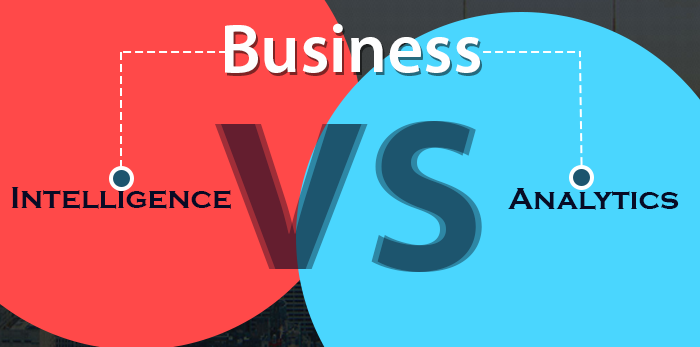
\includegraphics[width=13cm]{./Imagenes/image01}
\end{center}
\begin{center}
\textbf{Business Intelligence vs Business Analytics visto a través del fútbol}\\
\end{center}
\item 
Digamos que estás en el cuerpo técnico de un equipo de fútbol y quieres revisar el juego más reciente. Hace esto para ver cómo puede corregir sus errores y replicar sus éxitos.
\item 
Usando nuestras definiciones anteriores,  BI  sería el proceso de identificar todas las estadísticas y jugadas que llevaron a su equipo a ganar. Identificaría que mantuviste la posesión de la pelota por mucho más tiempo que tus oponentes. También identificaría la tendencia de que su lado derecho del campo fue fundamental para retener la posesión a través de pases excelentes.
\item 
El análisis de negocios  estaría más preocupado por la  razón por la  que tuvo posesión de la pelota por más tiempo que su oponente y por qué su lado derecho del campo le fue tan bien al pasar.
\item 
\item 
\textbf{Fue porque:}\\
\item 
- ¿Los defensores de tu oponente en ese lado eran jugadores más débiles que sus defensores en el otro?
\item 
- ¿Tus jugadores del lado derecho habían estado pasando más tiempo juntos en el campo que tu lado izquierdo?
\item 
- ¿Uno de tus jugadores de la derecha simplemente tenía un rendimiento fenomenal que se trasladó al resto de ese lado?
\item 
\item 
Estas preguntas son importantes. Le permiten descubrir cómo puede replicar su éxito o prevenir su fracaso en el futuro. Hacer las preguntas  correctas de inteligencia empresarial  lo llevará a mejores análisis. Al usar un tablero de negocios , todas las ideas se pueden simplificar en un solo lugar, haciendo que el tiempo para tomar decisiones significativas sea mucho más rápido. Pero primero, necesitamos analizar más la diferencia, ya que eso nos ayudará a comprender qué hacer en el proceso de operación de una empresa y cómo elegir la mejor herramienta para administrar sus conocimientos.
\item 
\textbf{¿Cómo se aplica esto a los negocios?}\\
\item 
¿Puede comprender los factores que están  causando  el éxito o el fracaso de su negocio en lugar de solo los factores  asociados  con el éxito o el fracaso de su negocio? Si es así, es mucho más probable que pueda predecir el futuro en su mercado y actuar en consecuencia. Sin embargo, es importante tener en cuenta que necesita saber qué está correlacionado con algo antes de poder conocer la causalidad.
\item
En otras palabras, debe saber  qué  sucedió y  cómo  sucedió (BI) antes de poder decir  por qué  sucedieron las cosas (BA) con un grado razonable de certeza.
\item
\item
\textbf{Escenarios de casos de uso}\\
\item
Solidifiquemos las cosas y terminemos esta publicación con ejemplos de negocios, ilustrando la diferencia entre inteligencia empresarial y análisis de negocios.
\item
Supongamos que trabaja para una empresa de marketing que utiliza inteligencia empresarial y análisis para ayudar a las grandes empresas de comercio electrónico a lanzar nuevos productos. Para comprender qué productos nuevos tendrían más probabilidades de tener éxito (análisis), necesitaría descubrir:
\item 
- Qué productos han tenido más éxito en el pasado (BI)
\item 
- Las tendencias estacionales que han influido en el éxito de lanzamientos anteriores (BI)
\item 
- Por qué los clientes compraron los productos exitosos del pasado (BA)
\item
\item
\begin{center}
\textbf{¿Qué diferencia existe entre el Business Intelligence y el Business Analytics?}\\
\end{center}
\item
\item
\textbf{Una mirada al pasado:}\\
\item
Business Intelligence (BI) permite visualizar y hacer análisis con base en la información histórica y es fundamental para que las empresas tomen decisiones, pues brinda un panorama de cómo se ha desarrollado históricamente un negocio. BI es también una categoría de aplicaciones y tecnologías para la recolección, almacenamiento, análisis y acceso a los datos para ayudar a los usuarios empresariales a tomar menores decisiones de negocios.
\item
\item
\textbf{La mirada al futuro:}\\
\item
Por su parte, Business Analytics (BA) se encarga de visualizar el futuro con base en la experiencia y la información y modelos predictivos que se conocen del negocio para anticiparse a las decisiones y
mejorar la competitividad. Es la practica de la explotación iterativa y metódica de datos de una organización con énfasis en el análisis estadístico y se utiliza para automatizar y optimizar los procesos de negocio.
\item
\item
\begin{center}
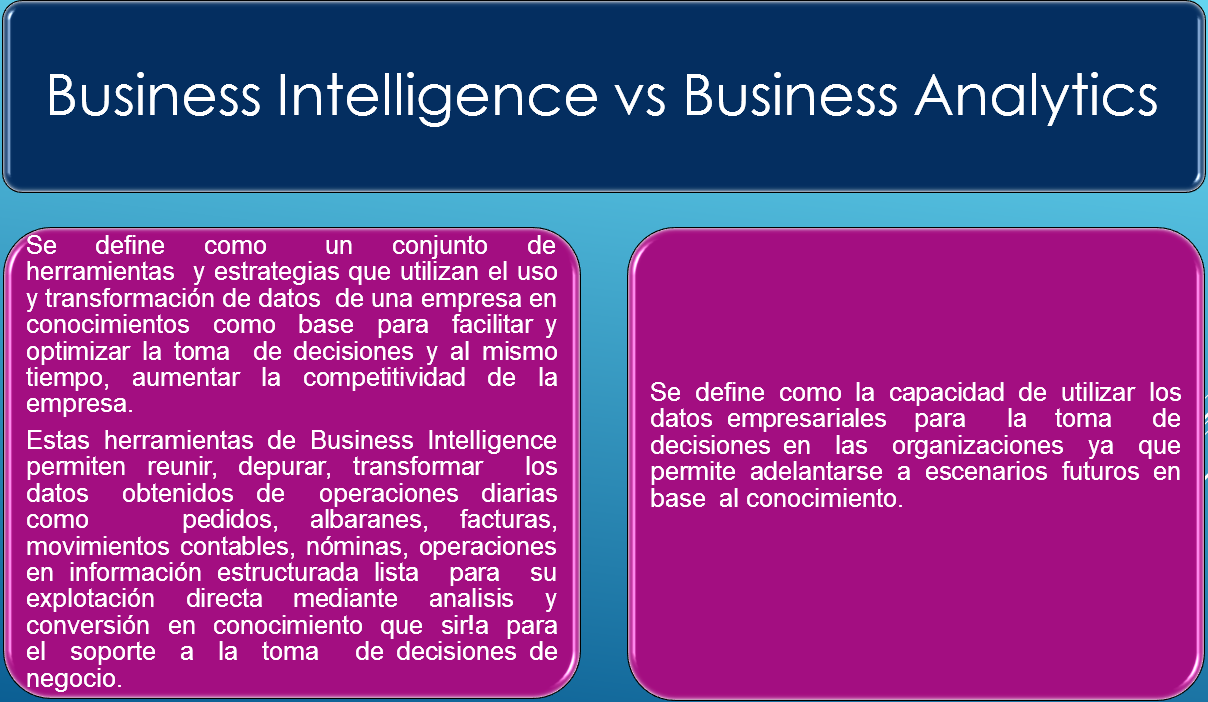
\includegraphics[width=17cm]{./Imagenes/image03}
\end{center}
\item
\item
\textbf{La gran  diferencia que existe entre el BI y BA, es que el Business Intelligence mira  hacia el pasado permitiendo visualizar y hacer analisis con base  en la información histórica para  ayudar a los usuarios empresariales a tomar menores decisiones de negocios, y el Business Analytics da una mirada hacia el futuro para  prevenir futuros problemas que puedan ocurrir en la empresa en  base  a la  experiencia e información  que  se  conocen del  negocio  para anticiparse a las decisiones y mejorar la competitividad.}

\item
\begin{center}
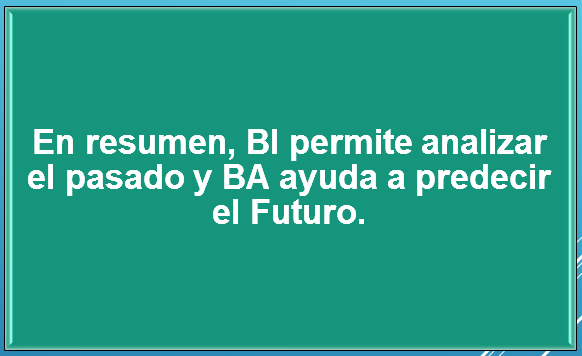
\includegraphics[width=13cm]{./Imagenes/image05}
\end{center}
\item

\begin{center}
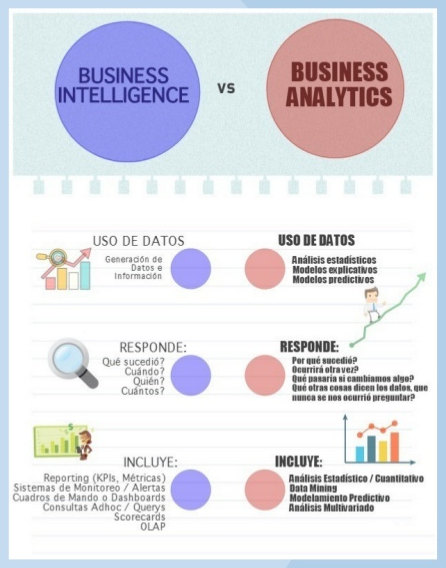
\includegraphics[width=15cm]{./Imagenes/image02}
\end{center}

\end{flushleft}
